\chapter{Marco Te\'orico}\label{chapter:theory}

\section{Asimetría hemisférica en humanos en la percepción de escalas espaciales}

Cuando se percibe una escena visual se procesan distintas escalas espaciales, recorriendo desde lo más global hasta los detalles locales.  Así podemos ver un bosque, pero también podemos ver los árboles que lo componen, y hasta las hojas de estos árboles [\cite{wagemans_perception_2014}] . Hay fuertes evidencias de que los dos hemisferios del cerebro juegan un papel distinto en este proceso [\cite{flevaris_spatial_2016}]. Se piensa que el hemisferio izquierdo es más eficaz en el procesamiento de detalles finos, mientras que el derecho sobresale en la percepción de patrones globales. Esto se ha estudiado experimentalmente con las figuras de Navon, en las cuales letras globales se componen de letras locales [\cite{navon_forest_1977}]. 
\begin{figure}[h]
	\centering
	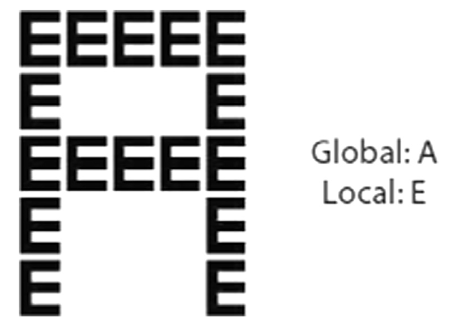
\includegraphics[scale=0.5]{Graphics/navon}
	\caption{Ejemplo de letra de Navon. Letra 'A' (global) compuesta por letras 'E' (local). Tomado de [\cite{flevaris_spatial_2016}]}
	\label{fig:navon}
\end{figure}
Al presentar letras de Navon [\cite{navon_forest_1977}] (Ver Figura \ref{fig:navon}), los observadores identifican más rápido la letra global cuando se presenta en el campo visual izquierdo (proyectado al hemisferio derecho) y más rápido la letra local cuando se presenta en el campo visual derecho (proyectado al hemisferio izquierdo) [\cite{navon_forest_1977}]. Por otra parte, los pacientes con lesiones en el hemisferio derecho tienen dificultades selectivas en la percepción de las letras globales, mientras que pacientes con lesiones en el hemisferio izquierdo tiene problemas para percibir elementos locales. Esta lateralización hemisférica se encuentra también en estudios de resonancia magnética funcional (fMRI, por sus siglas en ingl\'es) [\cite{han_hemispheric_2002}] y de electroencefalograf\'ia (EEG) [\cite{iglesias-fuster_asynchronous_2015}]. Sin embargo, todavía no existe un modelo ampliamente aceptado que explique el porqué y el cómo de esta laterización hemisférica.

\section{Papel de las frecuencias espaciales en la percepción visual}

El modelo más interesante para explicar la lateralización hemisférica de la percepción de la escala espacial, utiliza el concepto de las frecuencias espaciales de las imágenes [\cite{robertson_hemispheric_2000}]. Las imágenes visuales pueden descomponerse en componentes de variación más rápida o lenta, análogo a un análisis de series de Fourier. De hecho, el sistema visual actúa como si tuviera filtros de distintas frecuencias espaciales.

Distintas investigaciones [\cite{flevaris_local_2010}] sugieren que las frecuencias bajas se asocian con la percepción global, procesadas predominantemente por el hemisferio derecho, mientras que las frecuencias altas se vinculan con la percepción local, manejadas por el hemisferio izquierdo.

En experimentos donde los sujetos detectaban rejillas de distintas frecuencias espaciales se observó que eran más eficientes en la detección de rejillas de baja frecuencia espacial después de prestar atención a una letra de Navon global, mientras que eran más hábiles en la detección de rejillas de alta frecuencia después de focalizar su atención en las letras locales. Además, la identificación de las rejillas sinusoidales con líneas  ”más gruesas” era más eficiente en el hemisferio derecho, mientras que la identificación de líneas ”más delgadas” se detectaba mejor en  el hemisferio izquierdo [\cite{flevaris_local_2010}]. 

Basados en estas evidencias Robertson y colaboradores proponen el modelo del Doble Filtraje por Frecuencias [\cite{robertson_hemispheric_2000}]. En este modelo: (1) el sistema visual selecciona un rango de operación en el espacio de frecuencias espaciales, de acuerdo con la escena visual a analizar, y  después (2) distribuye la información a los dos hemiferios donde la banda de frecuencias más altas es filtrada por el hemisferio izquierdo y la banda de frecuencias más bajas, por el hemisferio derecho. Este modelo explicaría muchos de los hallazgos descritos arriba. Sin embargo, no postula un mecanismo en términos de circuitos neurales que puedan implementar las operaciones implicadas. El desarrollo de técnicas para estudiar el sistema visual con fMRI abre la posibilidad de identificar los circuitos neurales relevantes, tema que se aborda en la próxima sección.

\section{Resonancia Magn\'etica Funcional}

La resonancia magnética funcional (fMRI) es una técnica no invasiva para estudiar la activación cerebral con gran resoluci\'on espacial. Mide los cambios en la oxigenación de la sangre y el flujo sanguíneo relacionados con la actividad neuronal, ya sea en respuesta a una determinada tarea o en reposo. El método más popular para realizar fMRI utiliza el contraste dependiente del nivel de oxigenación sanguínea (BOLD, por sus siglas en ingl\'es), que aprovecha las diferencias en las propiedades magnéticas de la hemoglobina oxigenada y desoxigenada. Cuando hay mayor actividad neuronal en un sitio se incrementa el flujo de sangre oxigenada a este [\cite{lindquist_principles_nodate}]. El cambio derivado de esto en la señal de resonancia magnética se denomina función de respuesta hemodinámica (HRF, por sus siglas en ingl\'es).

Los datos adquiridos en un estudio de resonancia magnética funcional consisten en una secuencia de imágenes de resonancia magnética tridimensionales, cada una compuesta por una serie de elementos de volumen o vóxeles, uniformemente espaciados. Los vóxeles dividen el cerebro en una gran cantidad de cubos del mismo tamaño. Una imagen típica puede constar de aproximadamente 100.000 vóxeles, donde el valor de intensidad de la imagen correspondiente a cada vóxel representa la distribución espacial de la densidad del espín nuclear, que se relaciona con la oxigenación y el flujo de la sangre, en el área local. Durante un experimento de resonancia magnética funcional se obtienen entre 100 y 1.000 imágenes tridimensionales de todo el cerebro. 

Por tanto, fMRI resulta una herramienta ideal para examinar la organización de los circuitos neuronales en el hombre de forma no-invasiva, y en especial para ver los mecanismos neurales de la lateralización hemisférica de la percepción visual. Para ello vamos a utilizar el concepto de campo receptivo.

\section{Campos Receptivos de Poblaciones Neuronales}

El concepto de campo receptivo juega un papel central en el estudio de la vía visual. El campo receptivo de una neurona se refiere a la pequeña región en el campo visual donde una estimulación específica tiene el potencial de alterar la actividad de dicha neurona [\cite{kandel_principles_2021}]. Los primeros estudios de campos receptivos se realizaron con microelectrodos en la corteza de animales experimentales, lo que permitió identificar la arquitectura básica de las vías visuales. 

La evolución de esta perspectiva ha llevado a la conceptualización de los campos receptivos de población (pRF, por sus siglas en ingl\'es). Mientras que los campos receptivos convencionales describen las áreas específicas del espacio visual que activan una única neurona, los pRF se centran en la actividad de una población de neuronas [\cite{dumoulin_population_2008}]. Estos, constituyen modelos cuantitativos que predicen la actividad neuronal colectiva en un vóxel de fMRI y tienen en cuenta la selectividad de la respuesta neuronal en relación con la posición del estímulo en el espacio visual. La estimación de la posición y el tamaño de la sección del campo visual que afecta a un vóxel específico permite comprender cómo la población neuronal contenida participa en el procesamiento y representación de la información visual en el cerebro.

En [\cite{dumoulin_population_2008}] se f\'ormula un modelo matemático de pRF utilizando una función Gaussiana que describe cómo la respuesta neuronal varía con la distancia desde el centro del campo receptivo. Incluye parámetros como la posición del centro del pRF, su tamaño, y la magnitud de la respuesta. La función Gaussiana se ajusta a los datos de actividad neuronal, obtenidos a través fMRI, para estimar las características del pRF en una población neuronal específica. Este modelo se desarrolla en la próxima sección.


\section{Modelos matemáticos de campos receptivos de poblaciones neuronales}

En [\cite{zuiderbaan_modeling_2012}] se introduce un modelo de pRF basado en la función Diferencia de Gaussianas, mejorando la capacidad de representar respuestas inhibitorias y la supresión periférica en la corteza visual.

En [\cite{kay_compressive_2013}] se desarrolla un modelo de pRF con una no linealidad estática compresiva, es decir, reduce la amplitud de las respuestas a medida que aumenta la intensidad del estímulo. Este modelo explica que la respuesta total a estímulos múltiples es menor que la suma de respuestas individuales. En el modelo propuesto en [\cite{dumoulin_population_2008}] la estimación de los parámetros de los pRF se llevó a cabo utilizando datos de series temporales de respuestas de fMRI (Ver Fig 1.1). El modelo se basa en la suposición de una relación lineal entre los niveles de oxigenación de la sangre (BOLD) y las señales de resonancia magnética. Esta relación se expresa mediante la ecuación:
\begin{equation}
	y(t)=p(t)\beta + e
\end{equation}
donde $\beta$ es un factor de escala que tiene en cuenta las unidades desconocidas de la señal de fMRI y $e$ es el ruido de la medición. 

La predicción $p(t)$ se calcula utilizando un modelo parametrizado de la población neuronal subyacente y el estímulo. Se emplea un modelo gaussiano bidimensional $g(x,y)$ para describir la respuesta de la población neuronal, el cual est\'a definido por tres par\'ametros $x_0$,  $y_0$ y $\sigma$,
\begin{equation}
	g(x,y)=exp-(\frac{(x-x_0)^2+(y-y_0)^2}{2\sigma^2})
	\label{gaussian}
\end{equation}
donde ($x_0$,$y_0$) es el centro del pRF y $\sigma$ es la dispersión gaussiana o desviación estándar que caracteriza la extensi\'on del pRF. Estos parámetros están referidos a estímulos, por tanto, las unidades de $x_0$, $y_0$ y $\sigma$ están todas en grados de ángulo visual. La fórmula que describe el estímulo efectivo $s(x,y,t)$ es una función indicadora binaria que marca la posición de la apertura del estímulo en cada momento. La apertura del est\'imulo es la región específica de un estímulo visual que está siendo presentada o activada en un momento dado durante un experimento, por tanto, la función indicadora ser\'ia 1 en las posiciones dentro de la apertura y 0 fuera de ella.

Una vez obtenido un modelo de pRF determinado y un estímulo efectivo, se calcula la respuesta de pRF prevista. Dado que la fórmula de pRF (\ref{gaussian}) y la del estímulo efectivo se definen en las unidades comunes del espacio visual, para predecir la serie temporal de fMRI, es necesario calcular la superposición entre el estímulo efectivo y el modelo de pRF en un vóxel.

\begin{equation}
	r(t)=\sum_{x,y}s(x,y,t)g(x,y)
\end{equation}

Luego, se obtiene la predicción $p(t)$ de la serie temporal al convolucionar $r(t)$ con un modelo de HRF, el cual se estima por separado para cada sujeto.

\begin{equation}
	p(t) = r(t) * h(t)
\end{equation}

La bondad de ajuste se estima calculando la suma de cuadrados residual (RSS, por sus siglas en ingl\'es) entre la predicción, $p(t)$, y los datos, $y(t)$. Este término de error se calcula teniendo en cuenta un factor de escala, $\beta$, que tiene en cuenta las unidades desconocidas de la señal de fMRI.

\begin{equation}
	RSS = \sum_{t}(y(t)-p(t)\beta)^2
\end{equation}

Los parámetros óptimos de pRF se encuentran minimizando el RSS mediante una búsqueda de dos etapas de gruesa a fina (Ver [\cite{dumoulin_population_2008}] para m\'as detalles), enfoque que minimiza el tiempo de procesamiento y aumenta la probabilidad de encontrar un mínimo global. Se estiman tres parámetros del modelo pRF para cada vóxel de forma independiente: $x_0$, $y_0$ y $\sigma$. Estos, se hallan simultáneamente utilizando múltiples series temporales de fMRI medidas con varias aperturas de estímulo diferentes.

\begin{figure}
	\centering
	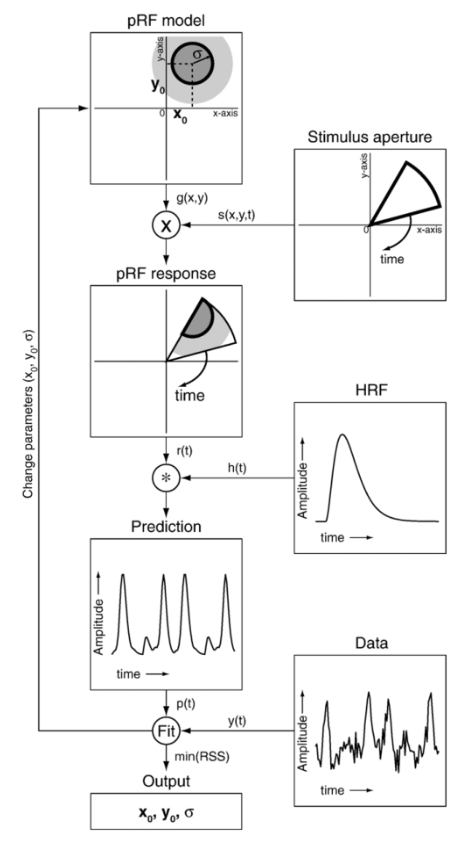
\includegraphics[scale=0.6]{../images/pRF model}
	\caption{Diagrama de flujo que describe el procedimiento de estimación del modelo pRF. Tomado de [\cite{dumoulin_population_2008}].}
	\label{fig:pRF}
\end{figure}

El ajuste de pRF permite derivar varias descripciones detalladas de los datos obtenidos. Entre ellas se encuentran los mapas tradicionales de excentricidad y ángulo polar, que revelan la disposición espacial y la orientación preferida de los campos receptivos en la población neuronal.

\section{Mapa Retinotópico}

La corteza visual humana está organizada en múltiples mapas retinotópicos [\cite{wandell_computational_2015}]. Un mapa retinotópico es una representación bidimensional de la superficie de la retina en una región específica del sistema visual del cerebro. En estos mapas se respeta la topología de la retina: ubicaciones cercanas en la retina se proyectan a áreas cercanas en la corteza. La corteza visual primaria (V1) es el punto de entrada de la información visual a la corteza, y el inicio de todas las rutas de procesamiento visual en el cerebro. En [\cite{benson_retinotopic_2012}] se demuestra que la topología superficial de la corteza occipital permite predecir con aceptable precisión la organización retinotópica de V1. Con medidas del ángulo polar y excentricidad de cada sitio de V1 (obtenidas con fMRI) se midió la localización de las respuestas neuronales en la corteza visual, y se desarrolló un modelo algebraico para ajustar estos datos. 

La mayoría de los análisis de mapas retinotópicos con datos de fMRI han utilizado este enfoque basado en vóxeles. El método general es: (1) medir las respuestas al mapeo de estímulos en la corteza; (2) derivar coordenadas retinotópicas para cada vóxel o vértice de superficie analizando ondas viajeras o resolviendo el modelo de campo receptivo de población (pRF) [\cite{dumoulin_population_2008}], descrito en la sección anterior, para cada vóxel; (3) finalmente se identifican límites de cada área mediante inspección visual.

Además de requerir mucho tiempo y esfuerzo, los mapas que resultan de este proceso conservan muchas fuentes comunes de error. Debido a las diversas fuentes de ruido, los mapas medidos tienen discontinuidades y a menudo omiten porciones del campo visual. Estas deficiencias del proceso de mapeo retinotópico tradicional se derivan del hecho de que se organizan en torno a la optimización del poder explicativo de las soluciones de retinotopía a partir de vóxeles individuales, en lugar de todo el campo visual o el área cortical. Como consecuencia, se producen mapas que no son uniformes ni completos, ni tienen en cuenta cómo el campo visual se deforma en la superficie cortical. Sin estos datos, la comparación de mapas entre sujetos es difícil y el examen cuantitativo preciso de las diferencias individuales es imposible.

Una alternativa al modelado de vóxeles de datos de fMRI es construir un atlas retinotópico, un modelo computacional del mapeo entre la posición del campo visual y la estructura cortical. Los atlas generalmente se crean basándose en una descripción promedio de la función en la superficie cortical de un grupo de individuos, por tanto, carecen de las diferencias individuales de los sujetos. Esto llevó al desarrollo de un m\'etodo bayesiano que se describe en la próxima sección.


\section{Mapa Retinotópico Bayesiano}

El método bayesiano propuesto aborda la necesidad de ajustar mapas retinotópicos a la corteza visual de sujetos individuales sin intervención humana. Utiliza un modelo bayesiano que combina datos, como mediciones de v\'oxeles o vértices retinotópicos en un sujeto, con un modelo previo basado en un atlas derivado de datos poblacionales previamente medidos (como el estudio de 181 sujetos hecho por el Human Connectome Project [\cite{benson_human_2018}]). La propuesta sugiere que este enfoque tiene el potencial de ofrecer descripciones más precisas de los mapas retinotópicos en sujetos individuales, en comparación con el uso exclusivo de un atlas o mediciones individuales. Se utiliz\'o la formulaci\'on bayesiana siguiente, donde la hipótesis $H$ es la deformación particular de la superficie cortical y la evidencia $E$ es un conjunto particular de mediciones retinotópicas.
\begin{equation}
	P(H|E) = \dfrac{P(E|H)P(H)}{P(E)}
\end{equation}


\section{Representaci\'on del tama\~no de los pRFs y de las frecuencias espaciales preferidas de los v\'ertices corticales en diferentes \'areas visuales}\todo{cambiar t\'itulo}

Con el propósito de obtener una comprensión de la visión humana, se realizan estudios que buscan caracterizar con precisión cómo los mapas retinotópicos, descritos en secciones anteriores, representan diversas propiedades visuales.

En [\cite{henriksson_spatial_2008}] se midieron curvas de sintonización de frecuencia espacial en áreas como V1, V2, VP, V3, V4v, V3A, y V5+, utilizando fMRI. Se observó que la frecuencia espacial óptima disminuye con el aumento de la excentricidad visual y varía según la ubicación retinotópica. Estos hallazgos apoyan la idea de que diferentes áreas visuales procesan la información visual en distintas escalas espaciales.

En [\cite{amano_visual_2009}] se analizan los mapas de campo visual y los tamaños de los pRF en el complejo MT+ humano, usando fMRI. Se halló que el tamaño de los pRF aumenta progresivamente desde V1/2/3 hasta LO-1/2 y TO-1/2, siendo TO-2 el área con los pRF más grandes. También observaron que, dentro de cada mapa, el tamaño de los pRF aumenta con la excentricidad.

En [\cite{silva_radial_2018}] se examina cómo la corteza visual humana representa el espacio visual. Se centra en las variaciones del tamaño de los pRF y el factor de magnificación cortical en diferentes ángulos polares en las áreas V1, V2 y V3 de la corteza visual. El factor de magnificaci\'on cortical es una medida de cuánto espacio en la corteza visual está asignado a percibir una unidad de área en el campo visual. Se encontr\'o que los cuadrantes derechos de las \'areas visuales V2 y V3 tienen tamaños de pRF más grandes que los cuadrantes izquierdos, pero con tamaños de efecto muy pequeños y que no hay una diferencia significativa en cuanto a cuadrantes en V1. \todo{annadir Silva}


En [\cite{aghajari_population_2020}] se aplica un modelo log-Gaussiano para estimar la sintonización de frecuencia espacial a nivel de cada vóxel cerebral, revelando cómo varía la sensibilidad a la frecuencia espacial en la corteza visual inferior. Se miden respuestas a estímulos visuales de diferentes frecuencias espaciales, a través de fMRI. Se analiz\'o la frecuencia espacial m\'axima promedio por rangos de excentricidad de \'areas visuales primarias en diferentes cuadrantes del campo visual. Los resultados indican que la frecuencia espacial preferida disminuye con la excentricidad visual y varía en función de la ubicación retinotópica. Además, se observa que el ancho de banda de sintonización depende de la excentricidad y está correlacionado con el pico de frecuencia espacial preferida.

En [\cite{kriegeskorte_understanding_2011}] se propone el desarrollo de modelos de campo receptivo en la corteza visual primaria utilizando fMRI. Critica los métodos convencionales como la medición de curvas de sintonización y la clasificación de patrones multivariados, y propone en su lugar la estimación del campo receptivo, método que permite medir respuestas a una amplia gama de estímulos y desarrollar modelos que describan cómo los estímulos se traducen en respuestas neuronales.

En [\cite{broderick_mapping_2022}] se desarrollaron modelos para analizar la sintonización de la frecuencia espacial en V1. Se ajustaron curvas de sintonización log-normal a las respuestas de grupos de vóxeles en diferentes excentricidades, que permiten estimar la respuesta promedio en la señal asociada con la dependencia del nivel de oxígeno en la sangre, en diferentes frecuencias espaciales. No se analiz\'o la lateralizaci\'on hemisf\'erica en V1 respecto a la preferencia de frecuencias espaciales de los v\'oxeles. Los resultados muestran que la frecuencia espacial preferida varía inversamente con la excentricidad y se ve influenciada por la orientación del estímulo. Constituye una ampliación a la investigación previa sobre la sintonización de la frecuencia espacial en la corteza visual humana, como la realizada por [\cite{aghajari_population_2020}].






